\documentclass{assignment}
\urlstyle{same}

\usepackage{listings} 
\let\verbatim\undefined 
\let\verbatimend\undefined 
\lstnewenvironment{verbatim}{\lstset{breaklines,basicstyle=\ttfamily}}{}
\linespread{1.5}

\author{Leigh Goetsch}
\prof{Dr. Turney}
\className{Systems Programming}
\classCode{CPE 2600}

\submissionDate{11/20/2024}
% \assignment{EX 4}
\title{Lab 10: Signals} 

\begin{document}
\maketitle
% \begin{multicols}{2}
% \raggedcolumns

\newpage


\section{Part 1: Signal Research}

\begin{itemize}
    \item \textbf{What is a signal disposition?} A signal disposition is the action that the operating system takes when a signal is delivered to a process.
    \item \textbf{What is a signal handler? What is it used for?} A signal handler is a function that is called when a signal is delivered to a process. It is used to handle the signal in a way that is specific to the process.
    \item \textbf{Name and describe each of the five (5) default dispositions?}
    \begin{itemize}
        \item \textbf{SIG\_DFL} - The default disposition for a signal is to terminate the process.
        \item \textbf{SIG\_IGN} - The signal is ignored.
        \item \textbf{SIG\_ERR} - The signal is ignored and an error is returned.
        \item \textbf{SIG\_HUP} - The signal is ignored and the process is terminated.
        \item \textbf{SIG\_STOP} - The process is stopped.
    \end{itemize}
    \item \textbf{Name and describe one way to programmatically send a signal to a process. Be able to give an example (the code) to send a signal.} One way to send a signal to a process is to use the \texttt{kill()} function. For example, to send a \texttt{SIGINT} signal to a process with a PID of 1234, you could use the following code:
    \begin{lstlisting}[language=C]
    kill(1234, SIGINT);
    \end{lstlisting}
    \item \textbf{Name and describe one way to send a signal to a process from the command line. Be able to give an example (the command, key combination, etc.) to send a signal.} One way to send a signal to a process from the command line is to use the \texttt{kill} command. For example, to send a \texttt{SIGTERM} signal to a process with a PID of 1234, you could use the following command:
    \begin{lstlisting}[language=bash]
    kill -SIGINT 1234
    \end{lstlisting}
\end{itemize}

\subsection{POSIX Signal Types}

\begin{itemize}
    \item \textbf{SIGINT}
    \begin{itemize}
        \item \textbf{Name and describe the signal} - The SIGINT signal is sent to a process when the user sends an interrupt signal (e.g., by pressing Ctrl+C).
        \item \textbf{Default disposition} - The default disposition for SIGINT is to terminate the process.
        \item \textbf{Can the disposition be overridden by a signal handler?} - Yes, the disposition can be overridden by a signal handler. This is because the process may want to handle the interrupt signal in a different way than the default behavior.
    \end{itemize}
    \item \textbf{SIGTERM}
    \begin{itemize}
        \item \textbf{Name and describe the signal} - The SIGTERM signal is sent to a process to request that it terminate.
        \item \textbf{Default disposition} - The default disposition for SIGTERM is to terminate the process.
        \item \textbf{Can the disposition be overridden by a signal handler?} - Yes, the disposition can be overridden by a signal handler. This is because the process may want to handle the termination signal in a different way than the default behavior.
    \end{itemize}
    \item \textbf{SIGUSR1}
    \begin{itemize}
        \item \textbf{Name and describe the signal} - The SIGUSR1 signal is a user-defined signal that can be used by a process for any purpose.
        \item \textbf{Default disposition} - The default disposition for SIGUSR1 is to terminate the process.
        \item \textbf{Can the disposition be overridden by a signal handler?} - Yes, the disposition can be overridden by a signal handler. This is because the process may want to handle the user-defined signal in a different way than the default behavior.
    \end{itemize}
    \item \textbf{SIGKILL}
    \begin{itemize}
        \item \textbf{Name and describe the signal} - The SIGKILL signal is sent to a process to force it to terminate immediately.
        \item \textbf{Default disposition} - The default disposition for SIGKILL is to terminate the process.
        \item \textbf{Can the disposition be overridden by a signal handler?} - No, it can't because the process must be terminated immediately.
    \end{itemize}
    \item \textbf{SIGSTOP}
    \begin{itemize}
        \item \textbf{Name and describe the signal} - The SIGSTOP signal is sent to a process to stop it from executing.
        \item \textbf{Default disposition} - The default disposition for SIGSTOP is to stop the process.
        \item \textbf{Can the disposition be overridden by a signal handler?} - No, it can't because the process must be stopped immediately.
    \end{itemize}
\end{itemize}


\section{Part 2: Working with a Signal Handler}

\subsection{SIGINT in signal\_handler.c}
\begin{figure}
    \centering
    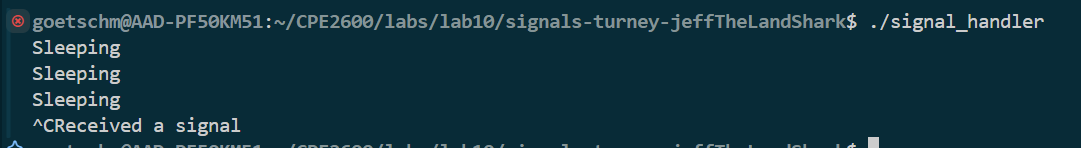
\includegraphics[width=1\linewidth]{images/SIGINT_ctrl_c.png}
    \caption{SIGINT triggered with CTRL + C}
\end{figure}

\begin{figure}
    \centering
    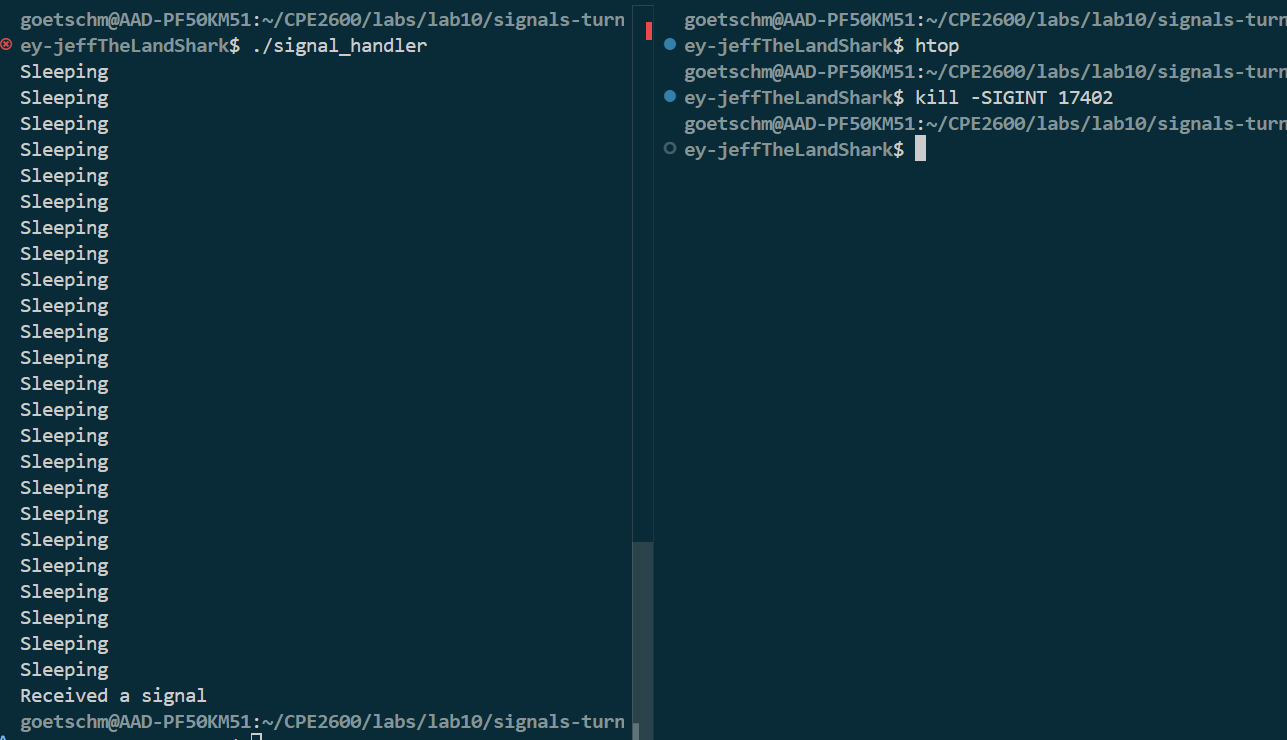
\includegraphics[width=1\linewidth]{images/SIGINT_kill.png}
    \caption{SIGINT triggered with kill cmd}
\end{figure}

\subsection{Exit Outside of Signal Handler}

\begin{figure}
    \centering
    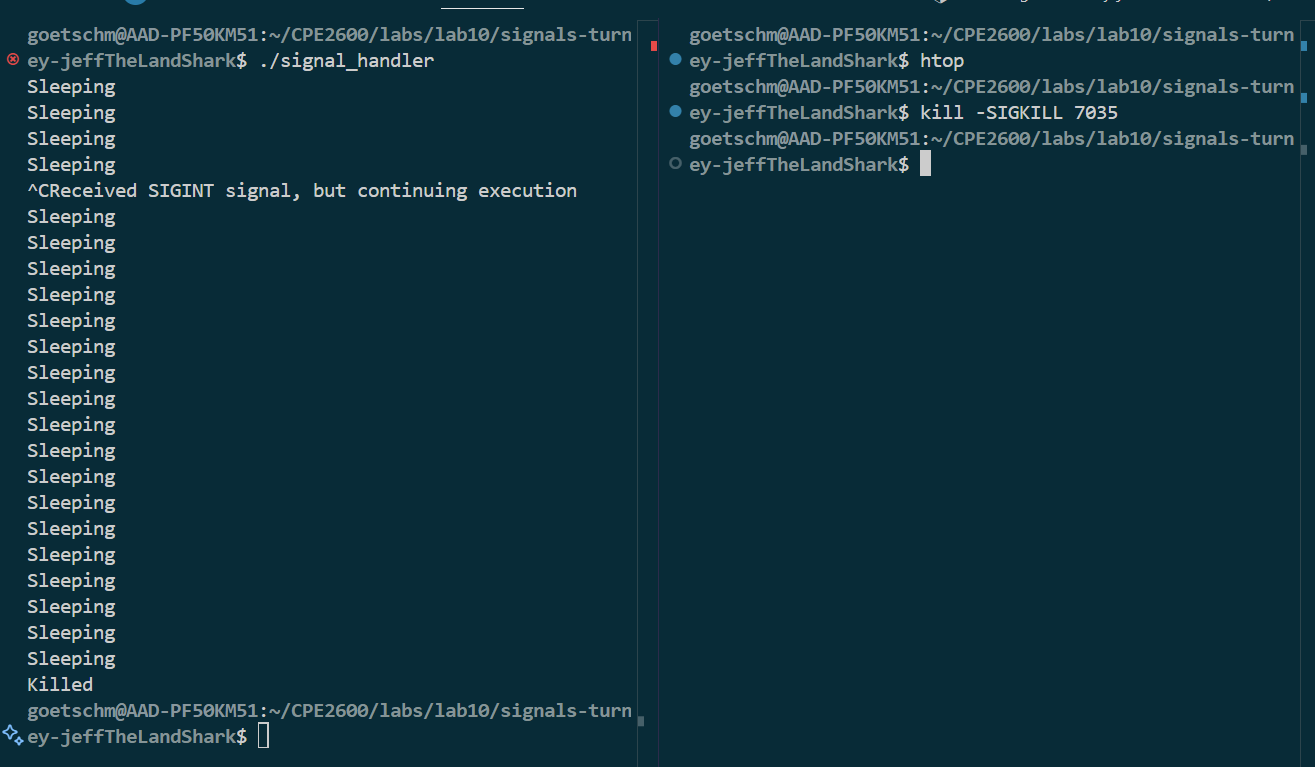
\includegraphics[width=1\linewidth]{images/SIGKILL.png}
    \caption{SIGKILL triggered with kill cmd, see how SIGINT doesn't close the program}
\end{figure}

\section{Part 3: Signals Sent From the Operating System}

\subsection{Using SIGALRM}
\begin{itemize}
    \item \textbf{The \verb|alarm| system call}\\
    Used to set an alarm for a specified number of seconds. When the alarm goes off, the process receives a \verb|SIGALRM| signal.
    \item \textbf{The \verb|SIGALRM| signal}\\
    Sent to a process when the alarm set by the \verb|alarm| system call goes off.
\end{itemize}

\begin{figure}
    \centering
    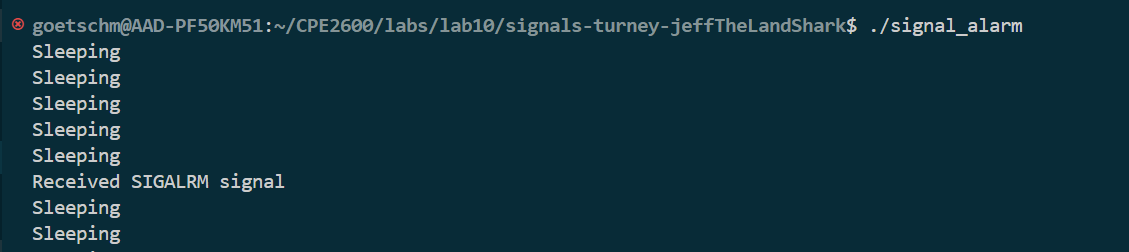
\includegraphics[width=1\linewidth]{images/SIGALRM.png}
    \caption{SIGALRM triggered with alarm system call}
\end{figure}

\subsection{Handling SIGSEGV}

\textbf{SIGSEGV} - sent to a process when it tries to access memory that it does not have permission to access.

\begin{figure}
    \centering
    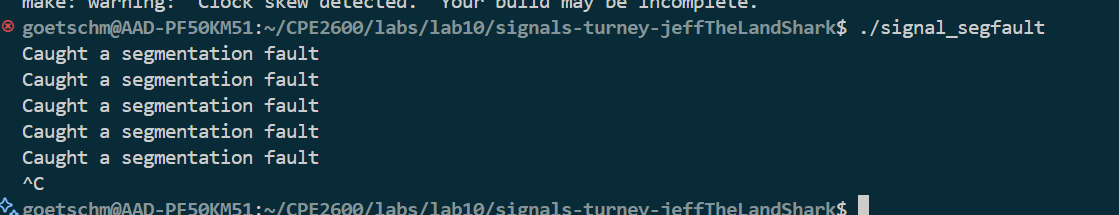
\includegraphics[width=1\linewidth]{images/SIGSEGV.png}
    \caption{Because SIGSEGV handles the signal but not the error, the program continuously sends the signal, resulting in an infinite loop}
\end{figure}



% \end{multicols}
\end{document}